%----------------------------------------------------------------------------------------
\begin{frame}
\begin{center}
\huge{Annexes}
\end{center}
\end{frame}

%---------------------------------------------------
\begin{frame}
\frametitle{An Exchange of mails really secure}

The problem with encrypted email? We still know who talks to whom.
\begin{block}{Solution}
\justifying{
\begin{itemize}
\item Exchange  mail between two  known / trusted servers who are dialoguing in https SSL / TLS between them.
\item Encrypt messages via PGP
\end{itemize}
}
\end{block}
\end{frame}

%---------------------------------------------------
\begin{frame}
\frametitle{Steganography - Steghide}

Can you see a difference between these two pictures?
\begin{figure}

\includegraphics[width=0.3\linewidth]{./materials/Steghide.jpg}
 vs

\includegraphics[width=0.3\linewidth]{./materials/Steghide.jpg}
\end{figure}
\justifying{
The second image contains the text "This is my hidden text." 
This is what is called steganography. Software : steghide
}
\end{frame}

%---------------------------------------------------
\begin{frame}
\frametitle{Bitmessage}
\justifying{
Bitmessage , a protocol for sending / receiving messages and acentric fully encrypted, based on a mechanism simillaire bitcoin .
}
\begin{figure}
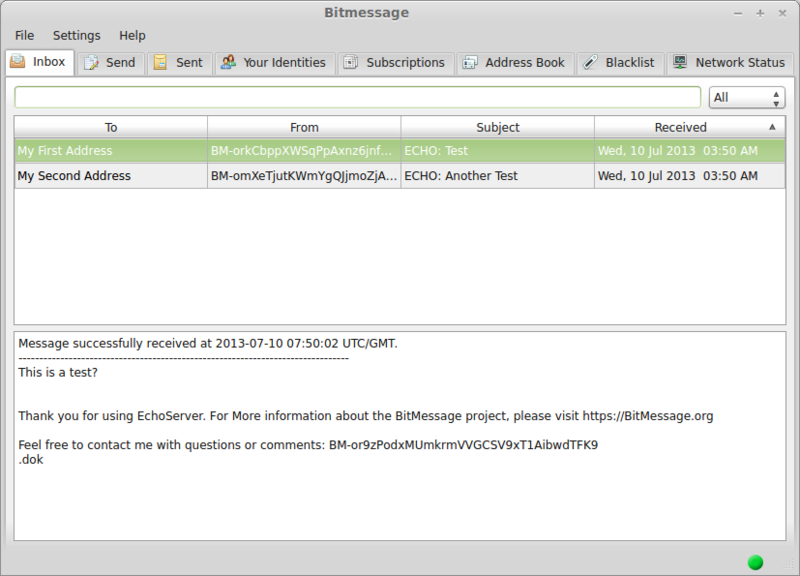
\includegraphics[width=0.7\linewidth]{./materials/Bitmessage.png}
\end{figure}
\end{frame}
	
\begin{frame}
\frametitle{Bitmessage}
\justifying{
Characteristics and comparison with an email solution + PGP
\begin{itemize}
\item Send a pair hand , no need to create a server, register a domain name, or enroll in a service. You can create as many addresses as you want.
\item No need to trust a tier ( CA for example).
\item Censorship-resistant . Person , including a government can not delete your address or messages.
\item It is not possible to impersonate a sender (spoofing).
\end{itemize}
}
\end{frame}

\begin{frame}
\frametitle{Bitmessage}
\justifying{
\begin{itemize}
\item Bitmessage has a feature broadcast .
\item The identity of the sender and receiver of messages is easier to hide an email with PGP + solution .
\item Unlike PGP , the subject is encrypted by default .
\item Should be easier to use, no need to keep the public keys of your correspondents .
\item Opportunity to develop additional functionality based on the protocol.
\end{itemize}
}
\end{frame}
	
%---------------------------------------------------
\begin{frame}
\frametitle{ZeroBin}

\justifying{
ZeroBin is a minimalist, opensource online pastebin/discussion board where the server has zero knowledge of hosted data. Data is encrypted/decrypted in the browser using 256 bits AES. You can test it online or install on your own server.
}
\begin{figure}
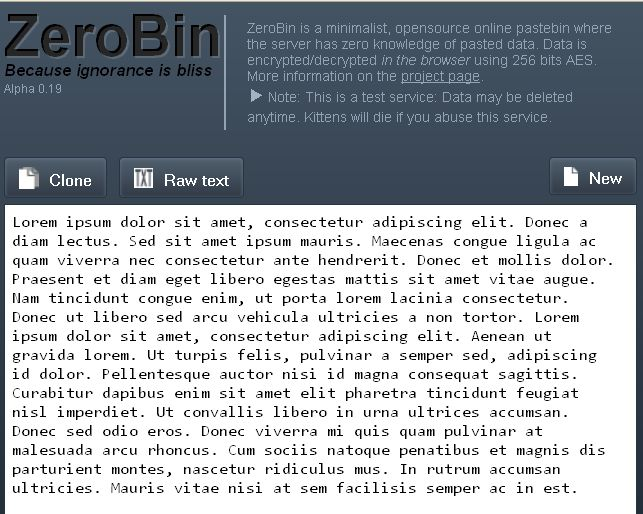
\includegraphics[width=0.5\linewidth]{./materials/Zerobin.jpg}
\end{figure}
\end{frame}

\begin{frame}
\frametitle{ZeroBin}
\begin{figure}
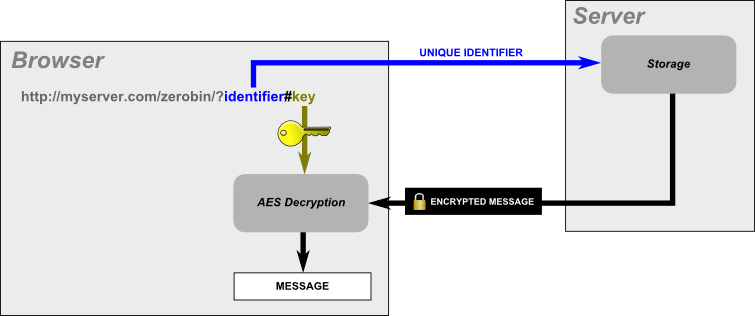
\includegraphics[width=0.8\linewidth]{./materials/zerobin_figure_decryption.png}
\end{figure}
\end{frame}

\begin{frame}
\frametitle{ZeroBin}
When pasting a text into ZeroBin:
\begin{itemize}
\item You paste your text in the browser and click the Send button.
\item A random 256 bits key is generated in the browser.
\item Data is compressed and encrypted with AES using specialized javascript libraries.
\item Encrypted data is sent to server and stored.
\item The browser displays the final URL with the key.
\item The key is never transmitted to the server, which therefore cannot decrypt data.
\end{itemize}
\end{frame}

\begin{frame}
\frametitle{ZeroBin}
\begin{figure}
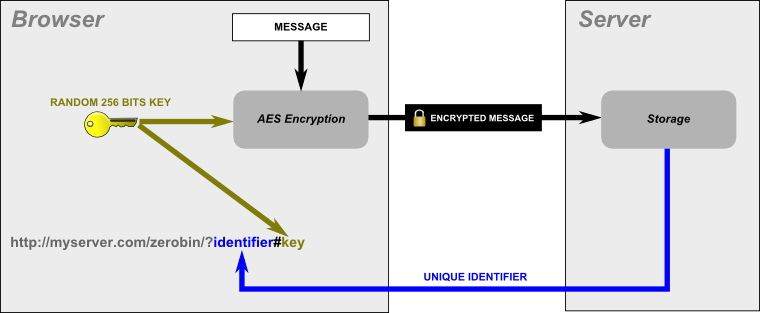
\includegraphics[width=0.8\linewidth]{./materials/zerobin_figure_encryption.png}
\end{figure}
\end{frame}

\begin{frame}
\frametitle{ZeroBin}
When opening a ZeroBin URL:
\begin{itemize}
\item The browser requests encrypted data from the server
\item The decryption key is in the anchor part of the URL which is never sent to server.
\item Data is decrypted in the browser using the key and displayed.
\end{itemize}
\end{frame}


